% chapter4 实验

\chapter{实验与结果分析}

\section{实验环境}

论文构建的HA-FuseNet是在实验室搭建的服务器上进行搭建和训练的,所用的软/硬件环境如表~\ref{tab:env}~所示:
\begin{table}[h]
    \centering
    \caption{实验环境}
    \label{tab:env}
    \begin{tabularx}{0.8\textwidth}{>{\centering\arraybackslash\hsize=0.6\hsize}X >{\centering\arraybackslash\hsize=1.4\hsize}X}
    \toprule
    软/硬件名称 & 型号/版本 \\
    \midrule
    操作系统 & Ubuntu 20.04.6 LTS  \\
    CPU & Intel(R) Xeon(R) Gold 5218R CPU @ 2.10GHz \\
    GPU & NVIDIA GeForce RTX 3090 \\
    内存 & 128GB \\
    显存 & 24GB \\
    CUDA & 11.8 \\
    Python & 3.11.5 \\
    Pytorch & 2.0.1 \\
    MNE & 1.6.0 \\
    Numpy & 1.26.3 \\
    \bottomrule
    \end{tabularx}
\end{table}

\section{数据与实验准备}

\subsection{运动想象脑电图数据集}

运动想象脑电图是使用脑电采集设备从头皮上获取的人类大脑的神经元活动时产生的生物电电位信号,能够反映大脑皮层和深层结构的功能状态及其异常变化。脑电图信号的采集过程主要包括以下几个步骤:

(1) 采集准备:根据国际10-20标准导联系统或其他标准定位方案,将电极安放在被试头皮的不同位置,以捕获不同脑区的电位信号。电极通常通过电极帽或电极盘固定,以确保位置的稳定和正确。由于人体脑电信号强度微弱,通常会通过与脑电采集设备相连的放大器对脑电信号进行增强和记录;

(2) 信号记录:当大脑神经元兴奋或抑制时,会产生微弱的电位变化,这些电位变化传导到头皮表面,形成可测量的电压差,由脑电采集系统进行捕获和放大。脑电采集系统通常以每秒连续进行\(N\)次采集的方式工作,即采集频率为\(N\)Hz;

(3) 数字化:根据脑电采集系统的设置,对被捕获的脑电信号进行一定的处理,包括通过模数转换器将模拟信号转换为数字信号。

在临床和科研应用中,脑电图信号因其非侵入性、实时监测性、对大脑功能活动的敏感性等特点,在大脑解码领域获得了广泛的应用。运动想象领域有多个公开的脑电图信号数据集,论文主要选取BCI Competition IV Dataset 2A数据集\cite{brunner2008bci}和BCI Competition IV Dataset 2B数据集\cite{leeb2008bci}作为模型训练和测试的数据集。脑机接口竞赛(BCI Competition)是一项由德国柏林洪堡大学和柏林工业大学发起的国际性脑机接口技术竞赛,旨在推动脑机接口技术的创新和发展。在第四届比赛(BCI Competition IV)中,主办方提供了多项数据集,其中,运动想象领域的BCI IV 2A和BCI IV 2B数据集在相关研究中被广泛使用。

\paragraph{BCI Competition IV Dataset 2A}

BCI Competition IV Dataset 2A数据集采集了9名被试的MI-EEG信号,包括4类运动想象任务,即左手、右手、双脚和舌头。每名被试在不同的日期进行了两次采集/会话(session),两个session分别被作为训练集(T)和测试集(E),数据以.gdf的格式存储,因此,每名被试具有两个文件,如对于一号被试而言,存在A01T.gdf和A01E.gdf两个文件,其中,训练集A01T.gdf包含标签信息,A01E.gdf不包含标签信息,使用额外的A01E.mat文件提供标签。

session采集的过程如图~\ref{fig:2asession}~所示,在采集开始时,进行约五分钟的EOG记录,包括两分钟的睁眼模式、一分钟的闭眼模式和一分钟的眼球运动模式。其中,四号被试的测试集只具有眼球运动的EOG记录。
\begin{figure}[ht]
    \centering
    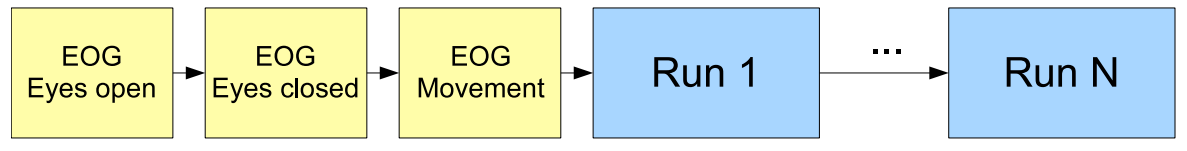
\includegraphics[width=0.7\textwidth]{2asession.png}
    \caption{2A session采集模式\cite{brunner2008bci}}
    \label{fig:2asession}
\end{figure}

在EOG记录之后,进行六次采集(run),在每个run中,各进行12次每类运动想象任务,这些任务的顺序是随机的,由此,一个run包含48次试验(trial),一个session包含288次试验(trial)。一个trial的流程如图~\ref{fig:2atrial}~所示,测试开始时(t=0s),一个十字图形出现在屏幕上,伴有简短的提示音;两秒后(t=2s),运动想象任务的指示箭头(分别指向左、右、下、上,对应左手、右手、双脚及舌头运动)出现在屏幕上,持续约1.25秒,每名被试进行运动想象任务直到十字图形消失(t=6s)。在这个过程中没有任何反馈。
\begin{figure}[ht]
    \centering
    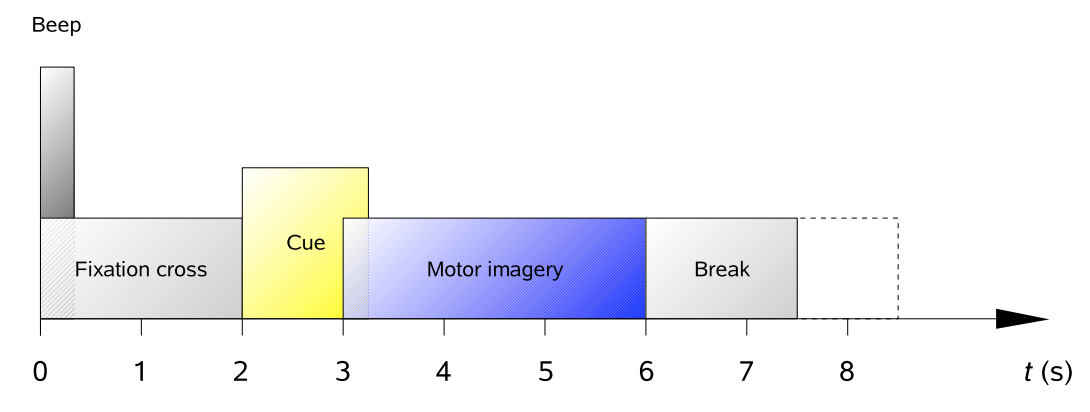
\includegraphics[width=0.7\textwidth]{2atrial.png}
    \caption{2A trial与无视觉反馈的2B trial的采集模式\cite{brunner2008bci,leeb2008bci}}
    \label{fig:2atrial}
\end{figure}

采集过程中,以250Hz进行EEG信号采样,并在0.5Hz至100Hz之间进行了带通滤波,放大器的灵敏度被设置为100\(\mu\)V,并使用了50Hz的陷波滤波器用以抑制线路噪声。头皮电极的位置按照国际10-20标准导联确定,共使用22个电极(通道),此外,还使用了3个不参与分类的EOG电极用以记录眼电信号。

在BCI领域,事件描述某一种波形或任务的起始点,数据上,事件表现为一个三元组:第一个元素以整数来描述的事件起始采样点;第二个元素对应当前事件来源的刺激通道的先前值,大多数情况下为0;第三个元素表示该事件的类型。BCI Competition IV Dataset 2A数据集中共包含11类事件,其中,与数据处理相关的事件如表~\ref{tab:2aevent}~所示,其中,拒绝试验是指由于质量欠佳或受试者未能有效完成任务而被专家标注出的试验数据。
\begin{table}[ht]
    \centering
    \caption{2A事件类型列表}
    \label{tab:2aevent}
    \begin{tabularx}{0.8\textwidth}{CC}
    \toprule
    事件类型 & 描述 \\
    \midrule
    768 & trial开始  \\
    769 & 左手运动想象任务(class 1) \\
    770 & 右手运动想象任务(class 2) \\
    771 & 双脚运动想象任务(class 3) \\
    772 & 舌头运动想象任务(class 4) \\
    783 & 未知运动想象任务(测试集) \\
    1023 & 拒绝试验 \\
    \bottomrule
    \end{tabularx}
\end{table}

论文遵循BCI Competition竞赛设置,使用T文件为训练集,E文件为测试集,针对每名被试进行被试内实验和被试间实验。则在不剔除拒绝试验数据的情况下,每名被试的训练集和测试集切片数量分别为:288,288。

\paragraph{BCI Competition IV Dataset 2B}

BCI Competition IV Dataset 2B数据集采取了类似BCI IV 2A数据集的采集方式,采集了9名被试的2类MI-EEG信号(左手、右手),每名被试在不同时间进行了五次session,数据以.gdf格式存储,每名被试有五个文件,例如,对于一号被试而言,B0101T.gdf、B0102T.gdf和B0103T.gdf为训练集,、B0104E.gdf和B0105E.gdf为测试集。其中,前两个文件不包含视觉反馈,后三个文件包含视觉反馈,即在试验过程中,通过屏幕上的笑脸图案对运动想象任务是否被正确执行予以反馈。无视觉反馈的session包含6次run,每个run包含20次trial(左手、右手各10次,随机排布),有视觉反馈的session包含4次run,每个run包含40次trial(左手、右手各20次,随机排布)。无视觉反馈的trial的采集模式与2A相同,如图~\ref{fig:2atrial}~所示。

BCI Competition IV Dataset 2B的事件类型与2A的事件类型相似,但不包含双脚和舌头运动想象任务。此外,不同于BCI IV 2A数据集的22个电极,BCI IV 2B数据集仅使用3个电极记录数据。

为了保证实验数据只涉及运动想象,而不涉及视觉反馈,论文选择无视觉反馈的两个session分别作为训练集和测试集,则在不剔除拒绝试验数据的情况下,每名被试的训练集和测试集切片数量分别为:120,120。

综上所述,论文所使用的数据的信息如表~\ref{tab:dataset}~所示。
\begin{table}[ht]
    \centering
    \caption{数据集信息}
    \label{tab:dataset}
    \begin{tabularx}{0.8\textwidth}{CCC}
      \toprule
      数据集 & BCI IV 2A & BCI IV 2B \\
      \midrule
      被试数量 & 9 & 9 \\
      类别数量 & 4 & 2 \\
      通道数量 & 22 & 3 \\
      频率范围 & 0.5-100Hz & 0.5-100Hz \\
      采样频率 & 250Hz & 250Hz \\
      训练集数据量 & 288(每被试) & 120(每被试) \\
      测试集数据量 & 288(每被试) & 120(每被试) \\
      \bottomrule
    \end{tabularx}
\end{table}

\subsection{数据预处理}

EEG信号具有低信噪比、非平稳、空间变异性等特性,并且通常具有较小规模的数据集,一般来说,对数据进行一定的预处理有助于后续分类任务。然而,论文基于端到端网络的思想构建模型,因此尽可能地对预处理操作进行削减。论文进行的数据预处理操作如下:

\paragraph{数据提取与切片}

MI-EEG原始信号储存在.gdf格式的文件中,除目标脑电信号之外,原始文件还包括EOG信号、间隙缺失值、与运动想象任务不直接相关的事件等。因此,在提取数据时,有必要进行一定的处理:

首先,剔除EOG通道数据,仅保留EEG通道数据,对于用于分隔run的缺失值(编码为非数字,NaN),使用对应通道的均值替代,以确保数据的连续性和完整性;

其次,对与运动想象任务直接相关的事件进行筛选和提取,并对相关时段进行切分。对于BCI IV 2A数据集、BCI IV 2B数据集,直接相关事件为四类运动想象任务事件或二类运动想象任务事件,并由提示信号(Cue)标识任务的开始,论文对连续数据进行切片,提取从Cue出现后的第1秒至第4秒(trial周期的第3秒至第6秒)的数据段,作为事件对应的运动想象任务持续期间产生的EEG信号,在后续加以分析。对于采样率为250Hz的数据集而言,3秒的数据区间将包含750个采样点。

需要说明的是,论文在数据提取过程中并未对拒绝试验进行剔除,同时未使用滤波器对EEG信号的频率进行过滤,以对真实应用情境中可能出现的多样化数据表现进行模拟,对模型自主识别各种频率成分并提取有效特征的能力进行评估。

\paragraph{标准化}

归一化操作的目的在于对数据的特征尺度进行统一,从而消除奇异数据导致的不良影响,提高模型的训练效率和稳定性。Z-score标准化、最大最小值归一化等方法是EEG信号处理中经典的算法。

经过Z-score处理的数据为标准正态分布,其操作过程如公式~\ref{eq:z-score}~所示。
\begin{equation}
    x=\frac{x-\mu}{\sigma}
    \label{eq:z-score}
\end{equation}
其中,\(x\)为原始数据,\(\mu\)表示\(x\)的均值,\(\sigma\)表示\(x\)的标准差。

最大最小值归一化的操作过程如公式~\ref{eq:maxmin}~所示,其是一种线性变换操作,将数据映射至\([0,\,1]\)区间,其中,\(X\)为一组通道数据。最大最小值归一化计算简单,但对具有波动性的EEG信号而言,将数据缩放至\([0,\,1]\)区间容易导致数据特征的损失。
\begin{equation}
    x=\frac{x-min(X)}{max(X)-min(X)}
    \label{eq:maxmin}
\end{equation}

因此,为了尽可能保留EEG信号的特征,论文应用Z-Score方法处理EEG信号,进行标准化,以提高模型训练的速度和稳定性。

\paragraph{数据增强}

MI-EEG信号通常具有较小规模的数据集,因此,通过一定的数据增强操作扩大数据规模,有助于提升网络训练效果,防止过拟合现象的发生。然而,在BCI系统的实际应用中,数据增强操作可能会导致训练阶段数据处理压力的增长,因此,在论文中,数据增强是一项可选操作,其目的在于提高模型分类精度,论文将分别使用进行数据增强和不进行数据增强的数据集进行训练。

EEG信号的数据增强方法主要有以下几种:

(1) 添加随机噪声:在EEG信号上叠加高斯白噪声、有色噪声等不同类型的噪声,模拟真实环境中的噪声干扰,能够提升模型的抗噪性和鲁棒性;

(2) 滑动窗口:设定时间滑动窗口的长度小于运动想象任务持续的时间长度,将滑动窗口内的数据视作一次事件,通过滑动窗口对数据进行切片,有助于模型学习EEG信号随时间变化的特征;

(3) 频率混叠:在保持EEG信号特性的前提下,将多种不同频率成分进行混叠,使得模型能够学习更广泛的频率特征。

由于在预处理阶段没有采取频率滤波的操作,论文采取频率混叠的方式对EEG信号进行增强,从而加强模型识别不同频率成分的能力。具体算法流程如算法~\ref{alg:aug}~所示。
\begin{algorithm}[H]\label{alg:aug}
    \caption{数据增强算法}
    \SetAlgoLined
    \KwData{Dataset for every subject $X=\{x_1, x_2, ..., x_9\}$ and the $subject\_id$ to be augmented.}
    \KwResult{augmented dataset for every subject $Y=\{y_1, y_2, ..., y_9\}$.}
    $Y = []$ \;
    \For{each item $x_i \in X$}{
        $X' = $ selected $x_j$ from $X,\,j \neq i,\,j \in [1,2,...,9]$ \;
        $y_i = x_i$ \;        
        $x_i = $ crop $x_i$ from where the first trial begins\;
        $x_i = $ filter $ x_i $ into $ [4Hz,40Hz] $ \;
        \For{each item $s_i \in X'$}{
            $s_i = $ crop $s_i$ from where the first trial begins\;
            $s1_i = $ filter $ s_i $ into $ [0.5Hz,4Hz)$ \;
            $s2_i = $ filter $ s_i $ into $ (40Hz,100Hz)$ \;
            $y_i = $ concatenate $ (y_i, s1_i+x_i+s2_i)$ \;
        }
        $Y = Y$ append $y_i$ \;
    }
    \Return{$Y$}\;
\end{algorithm}

\subsection{实验准备}

\paragraph{评价指标}

论文主要使用准确率(Accuracy,Acc)、Kappa一致性系数(Kappa)和标准差(Standard Deviation,SD)作为模型的评价指标。其中,准确率是分类任务中常用的评价指标,用于衡量模型预测结果与真实标签相匹配的比例,其计算方式为总样本中,分类正确的样本的比例。

Kappa一致性系数用于衡量模型预测结果与真实标签之间的一致性程度,在类别不平衡或随机猜测具有一定效果的情况下,Kappa一致性系数尤其有效。Kappa系数基于混淆矩阵进行计算,其计算公式如~\ref{eq:kappa}~所示。
\begin{equation}\label{eq:kappa}
    Kappa=\frac{P_o-P_e}{1-P_e}
\end{equation}
其中,\(P_o\)为观察一致性(Observed Proportion of Agreement),即准确率,\(P_e\)为预期一致性(Expected Proportion of Agreement by Chance),假设样本总量为\(N\),类别总量为\(c\),第\(i\)类的真实样本个数为\(x_i\),预测样本个数为\(p_i\),则\(P_e\)的计算公式如~\ref{eq:pe}~所示。
\begin{equation}\label{eq:pe}
    P_e=\frac{\sum_{i=1}^{c}x_i \times p_i }{N^{2} } 
\end{equation}
Kappa系数的范围在-1至1区间内,通常大于0,Kappa值越大,表明一致性程度越高,当Kappa值位于[0.61,0.80]区间时,表示预测与真实具有高度的一致性。

标准差为准确率的标准差,用于衡量模型在不同被试之间的稳定性能力,其值越小,表明不同被试的准确率越相近,模型在不同被试间的性能表现越稳定。准确率标准差的计算方式如公式~\ref{eq:sd}~所示。
\begin{equation}
    SD=\sqrt{\frac{1}{N-1}  \sum_{i=1}^{N}(x_i-\bar{x} )^{2} } 
    \label{eq:sd}
\end{equation}
其中,\(N\)表示被试数量,\(x_i\)表示第\(i\)个被试的准确率,\(\bar{x}\)为\(N\)个被试准确率的平均值。

\paragraph{损失函数及参数配置}

论文使用交叉熵损失函数(Cross Entropy Loss)。交叉熵用于度量预测概率分布与实际概率分布之间的不一致,其值越小,表明两个概率分布越相似,因此,可以通过最小化交叉熵的方式,使得一个概率分布逼近目标概率分布。

交叉熵损失函数是一类在分类任务中广泛应用的损失函数,能够衡量模型预测值与真实标签之间的差异,其计算如公式~\ref{eq:loss}~所示。
\begin{equation}
    L= -\sum_{i=1}^{C}y_i log(\hat{y}_i )
    \label{eq:loss}
\end{equation}
其中,\(C\)为分类类别数,\(y_i\)表示真实类别,\(\hat{y}_i\)表示模型预测的类别\(i\)的概率。交叉熵损失函数使用真实标签对模型预测的结果进行惩罚,从而促使模型学习到更为准确的预测结果。

论文使用Adam优化算法。对于BCI IV 2A数据集,批大小设置为32,BCI IV 2B数据集设置为20;实验迭代次数设置为300次;学习率的初始值设置为1e-3,权重衰减值设置为5e-3。

\section{实验设计}

\subsection{DIS-Net实验设计}

为了确定模型架构的最佳设置,本节对DIS-Net构建过程中不同的模型架构进行实验,从而逐步构建起性能最优的模型。

\paragraph{基础网络}

为了验证Inception\cite{szegedy2015going}、ResNet\cite{he2016deep}与U-Net\cite{ronneberger2015u}在MI-EEG分类任务中的性能,论文在BCI Competition IV Dataset 2A数据集上进行实验对比。在实验设置中,统一将三种模型的网络深度调整为三层,并对其他关键参数如卷积核大小进行了固定,此外,对这三种模型的原始代码进行了调整,使得其适应MI-EEG分类任务。实验结果如表~\ref{tab:Incep-Res-U}~所示,其中,准确率和Kappa系数是数据集中九位被试的平均表现。
\begin{table}[ht]
  \centering
  \caption{Inception、ResNet、U-Net实验结果对比}
  \label{tab:Incep-Res-U}
  \begin{tabularx}{\textwidth}{CCCC}
    \toprule
    模型 & ACC(\%) & Kappa & SD\\
    \midrule
    ResNet & 56.94 & 0.43 & \textbf{11.96}\\
    U-Net & 62.27 & 0.50 & 12.10 \\
    Inception* & \textbf{67.40} & \textbf{0.56} & 16.15\\
    \bottomrule
  \end{tabularx}
\end{table}

从准确率和一致性分析,Inception模型在这三种模型中具有最优的性能表现,U-Net次之,ResNet的表现则相对较差。这可能是因为同样的网络深度下,Inception模型得益于多尺度并行特征提取机制,能更全面地捕获EEG信号的多种特征。相比之下,U-Net虽然通过跳跃连接有效地结合了EEG信号的低层特征和高层语义信息,但在解码器阶段,U-Net将特征图重建至原始空间尺寸的过程可能为分类任务引入了不必要的复杂性。ResNet的快捷连接在较浅层网络结构中可能未能完全发挥其优势,更适用于深层次网络。实验结果与过往研究中关于浅层网络能够在MI-EEG分类任务中取得良好性能的研究结论相互印证。从准确率标准差分析,ResNet具有最优的跨被试稳定性,U-Net次之,然而,考虑到准确率与Kappa一致性的明显差异,论文仍然选择Inception模型为网络构建的基础,并通过一系列改进优化准确率标准差。

\paragraph{Inception模块引入空间卷积层的方式}

在DI-Net中,空间卷积层有两种不同的方式融入基于Inception改进的时间卷积层之后,一种是在每个Inception模块内部的分支结构上增加空间卷积层,另一种则是在整个Inception模块之后附加空间卷积层。图~\ref{fig:ts-incep}~展示了这两种引入方式的区别,将这两种方式分别称为分支内融合(Inception-In)和模块后融合(Inception-After),需要说明的是,图中省略了网络的其他结构,如瓶颈层等,以尽可能简洁地展现不同引入方式的差异。其中,\(s\_kernel\)表示空间卷积核,\(t\_kernel_i\)表示第\(i\)个分支的时间卷积核。
\begin{figure}[ht]
  \centering
  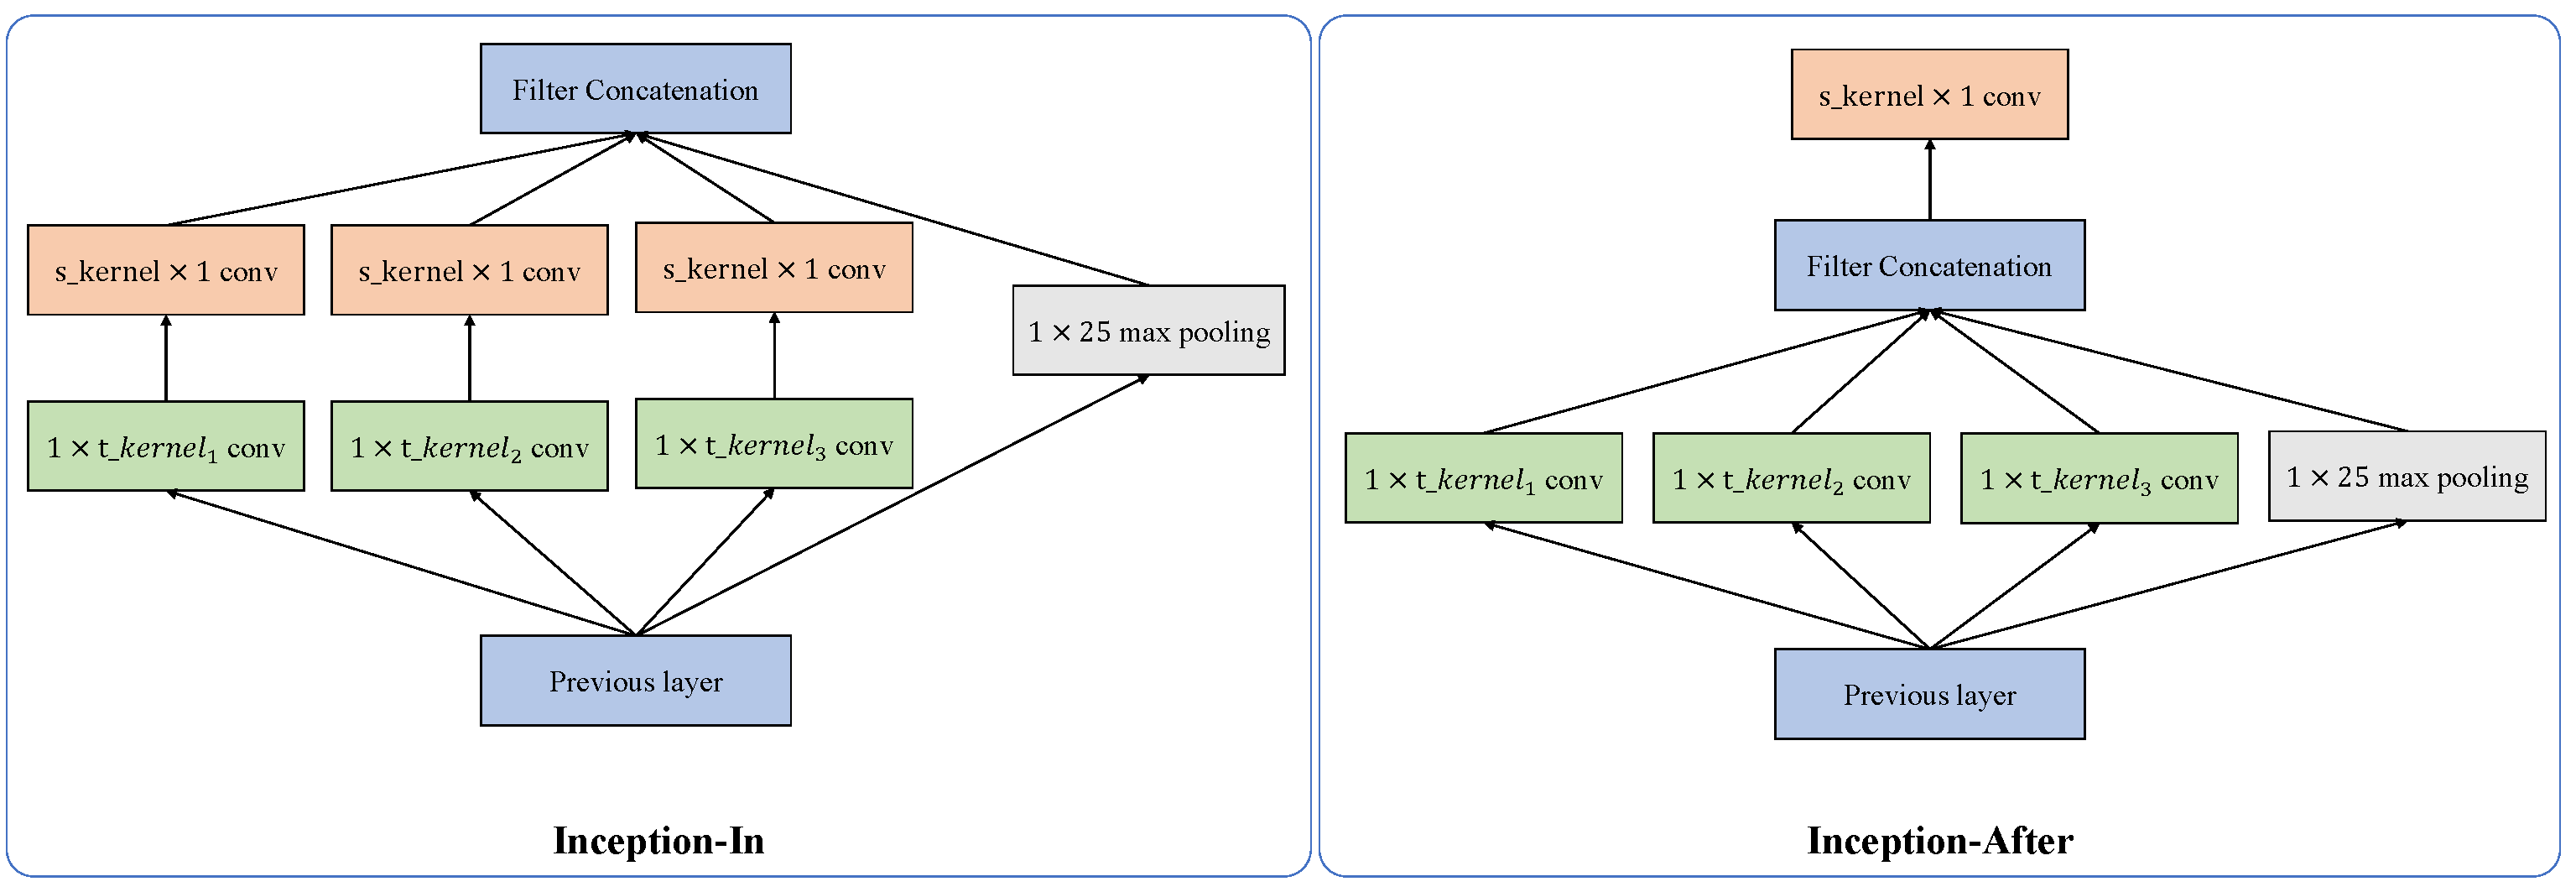
\includegraphics[width=\textwidth]{ts-incepv3.pdf}
  \caption{Inception模块引入空间卷积层的方式}
  \label{fig:ts-incep}
\end{figure}

为了比较Inception-In与Inception-After的性能差异,论文在BCI Competition IV Dataset 2A数据集上设计实验进行对比。在实验设置阶段,固定了Inception模块的层次数量、分支数量等参数,实验结果如表~\ref{tab:ts-inception}~所示。表格中的准确率与Kappa值均为数据集中九位被试的平均表现。实验结果显示,Inception-After方式在准确率、Kappa一致性系数、准确率标准差上均表现更优。这一优势可能源自两方面的原因:一方面,虽然Inception-In模式借鉴了FBCSP算法的分频段处理思路,但在Inception分支内部直接进行空间特征提取的过程中,损失了部分空间全局信息;另一方面,Inception-In结构具有相对更大的参数规模,这可能导致模型在有限样本条件下更容易出现过拟合现象。基于以上分析和实验验证,论文选择以Inception-After的方式布局时间卷积层与空间卷积层。
\begin{table}[ht]
  \centering
  \caption{Inception-In、Inception-After实验结果对比}
  \label{tab:ts-inception}
  \begin{tabularx}{\textwidth}{CCCC}
    \toprule
    模型 & ACC(\%) & Kappa & SD \\
    \midrule
    Inception-In & 69.01 & 0.58 & 14.44 \\
    Inception-After* & \textbf{74.42} & \textbf{0.65} & \textbf{11.92}\\
    \bottomrule
  \end{tabularx}
\end{table}

\paragraph{svSE模块引入的对比实验}

为了选择适合MI-EEG分类任务的基准注意力机制,论文在DI-Net引入了不同的混合注意力模块,并在BCI IV 2A数据集上进行了实验,实验结果如表~\ref{tab:att}~所示,表中的准确率和Kappa系数为九位被试的平均表现。数据显示,在三项指标上,scSE模块都取得了最好的表现,因此论文选择基于scSE模块进行改进。
\begin{table}[ht]
    \centering
    \caption{不同注意力模块引入DI-Net的实验结果对比}
    \label{tab:att}
    \begin{tabularx}{\textwidth}{CCCC}
      \toprule
      注意力模块 & ACC(\%) & Kappa & SD \\
      \midrule
      CBAM\cite{woo2018cbam} & 74.97 & 0.64 & 11.70 \\
      CoordAttention\cite{Hou2021CoordinateAF} & 73.82 & 0.62 & 12.16\\
      scSE\cite{8578843} & 75.35 & 0.67 & 11.58 \\
      svSE* & \textbf{76.16} & \textbf{0.68} & \textbf{11.33} \\
      \bottomrule
    \end{tabularx}
\end{table}

在表~\ref{tab:att}~中,同样展示了svSE以同样方式引入DI-Net的效果,svSE在四类混合注意力机制中取得了最高的准确率和Kappa系数,准确率标准差则为最低,证明了svSE模块针对EEG信号的特性进行的改进的有效性。

DIS-Net中,由于DI-Net的特征提取过程分为时间卷积和空间卷积两个阶段,svSE模块可采取以下三种引入方式:其一是在时间卷积层后引入;其二是在空间卷积层后引入;其三是同时在时间卷积层和空间卷积层之后引入。图~\ref{fig:att-Base}~展示了这三种引入svSE模块的方式,从左至右分别是时间卷积层后引入svSE模块、空间卷积层后引入svSE模块,以及在时间卷积和空间卷积层后均引入svSE模块。将这三种引入方式对应的模型分别简称为S-Temporal-Net、S-Spatial-Net、S-TS-Net。
\begin{figure}[ht]
  \centering
  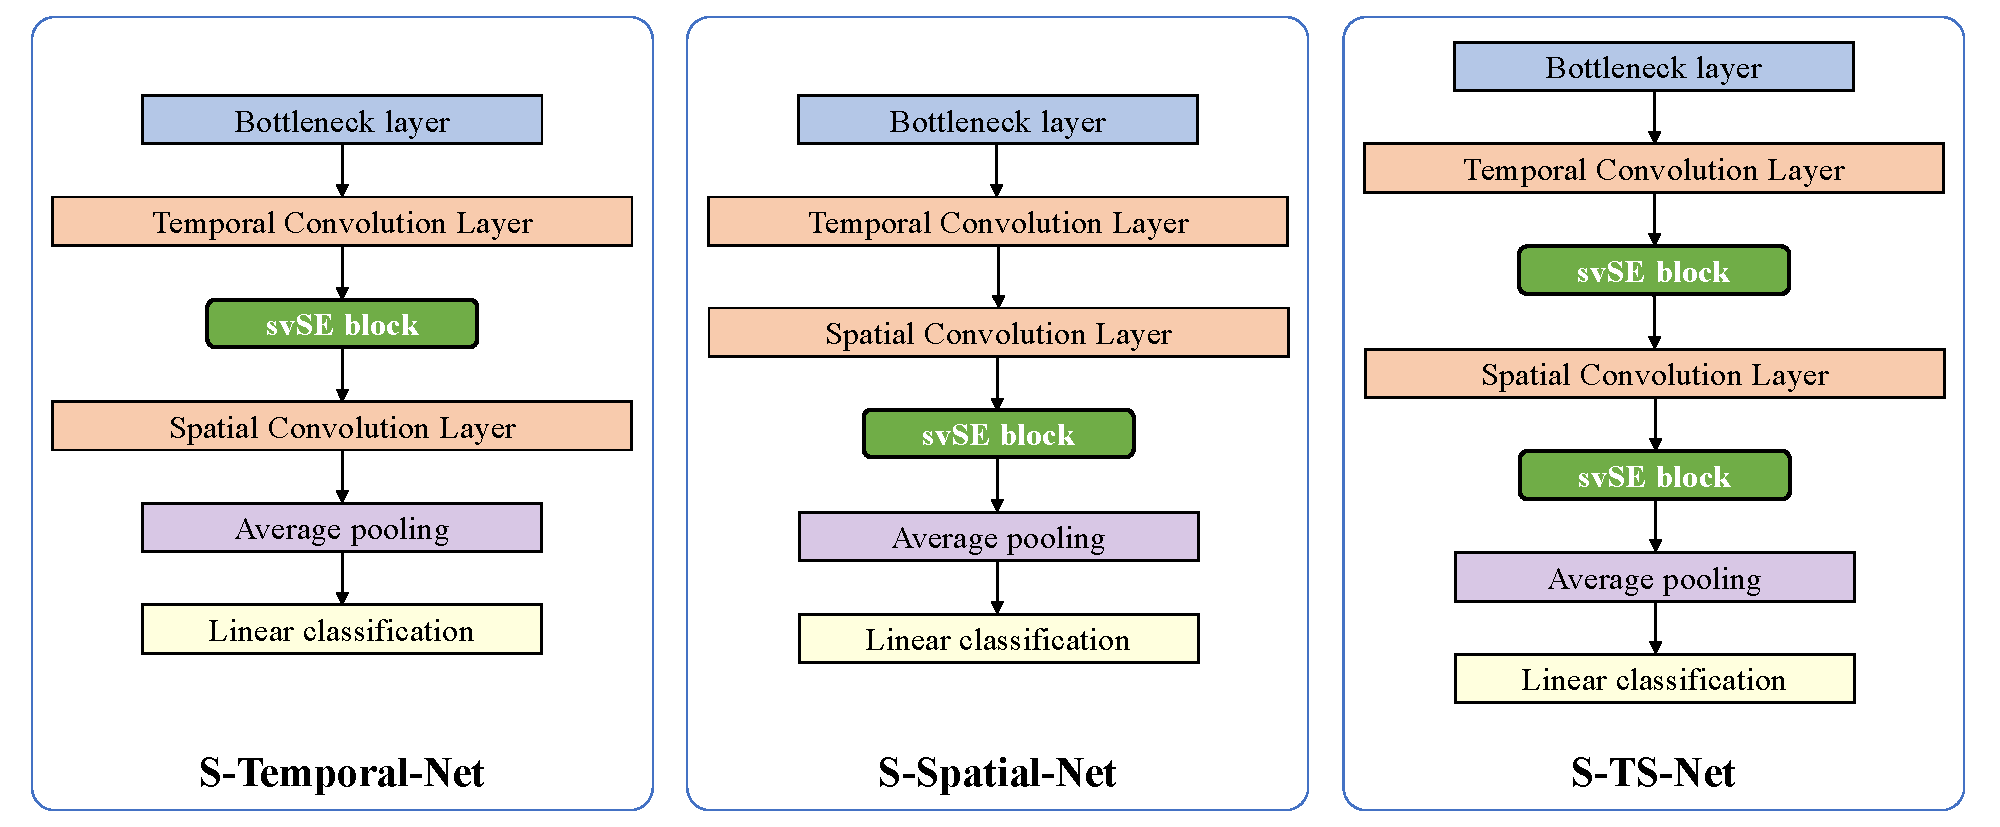
\includegraphics[width=\textwidth]{att-Basev2.pdf}
  \caption{DI-Net引入注意力模块的方式}
  \label{fig:att-Base}
\end{figure}

表~\ref{tab:svSE-BaseNet}~展示了S-Temporal-Net、S-Spatial-Net、S-TS-Net三种模型在BCI IV 2A数据集上的对比实验结果。表格中的准确率和Kappa系数为数据集中九位被试的平均表现。从准确率和一致性分析,S-ST-Net模型的效果优于其他两种模型,与经验相符。此外,S-Temporal-Net模型的效果优于S-Spatial-Net模型,其原因可能在于,空间卷积层沿通道维度的卷积使得数据损失了部分特征,进而减弱了svSE模块提取关键特征权重的能力,而时间卷积层保留了大部分深度信息和通道信息,因此,在时间卷积层之后加入svSE模块能够帮助模型更好地捕捉深度和空间的特征。从标准差分析,S-TS-Net模型的准确率波动幅度较小,对不同被试的MI-EEG分类效果相对均衡,另外两种模型在不同被试间的分类精度则存在较为明显的差异。实验数据显示,S-TS-Net模型取得了更好的效果,因此,论文采用了同时在时间卷积层和空间卷积层之后引入svSE模块的方式,即DIS-Net。
\begin{table}[ht]
    \centering
    \caption{svSE模块引入位置对比}
    \label{tab:svSE-BaseNet}
    \begin{tabularx}{\textwidth}{CCCC}
        \toprule
        模型 & ACC(\%) & Kappa & SD \\
        \midrule
        S-Temporal-Net & 76.09 & 0.68 & 11.57 \\
        S-Spatial-Net & 75.03 & 0.66 & 11.88 \\
        S-TS-Net* & \textbf{76.16} & \textbf{0.68} & \textbf{11.33} \\
        \bottomrule
    \end{tabularx}
\end{table}

\paragraph{不同轻量化模块对比}

为了验证更适合的轻量化卷积模块,论文在BCI Competition IV Dataset 2A数据集上进行了实验验证。由于轻量化卷积主要针对密集连接进行改进,实验使用DI-Net,并固定了Inception层数、密集连接层数、\(ratio\)等超参数。对\(ratio\)进行固定而非设置为可训练参数的原因是控制模块参数量的大小,避免轻量化卷积模块向未经轻量化的密集连接模块趋近。表~\ref{tab:lite}~展示了ShuffleNet、GhostNet、SG和未经轻量化的密集连接模块(Dense)的对比实验结果,其指标为参数量(Parameters)、浮点运算数(Floating Point Operations,FLOPs)和准确率,其中,准确率为九位被试的平均值。
\begin{table}[ht]
    \centering
    \caption{轻量化卷积模块实验结果对比}
    \label{tab:lite}
    \begin{tabularx}{\textwidth}{CCCC}
      \toprule
      轻量化卷积 & Paramters(K) & FLOPs(M) & ACC(\%) \\
      \midrule
      Dense & 29.99 & 690.37 & 74.42\\
      ShuffleNet & 7.31 & 130.37 & 72.96\\
      GhostNet & \textbf{7.27} & \textbf{129.93} & 73.14\\
      SG* & 7.36 & 133.04 & \textbf{73.71}\\
      \bottomrule
    \end{tabularx}
\end{table}

数据显示,ShuffleNet的轻量化效果较GhostNet较差,因此,论文选择基于GhostNet进行改进。这可能是因为相较于ShuffleNet,GhostNet对特征图的处理更充分,且引入了\(ratio\)参数用以控制不同操作分支的特征图的数量,相较于ShuffleNet具有更好的灵活性。在表~\ref{tab:lite}~中,GhostNet具有最优的轻量化效果,而SG模块在三种轻量化模块中取得了最优的性能,超越了GhostNet和ShuffleNet,这证明了对GhostNet改进的有效性,即使用可分离卷积与逐点卷积能够促进特征图之间的交互,从而更好地对特征进行拟合。

实验证明,相较于未经轻量化的密集连接模块,SG模块的轻量化效果明显;相较于GhostNet、ShuffleNet,SG模块取得了更优的性能。这证明了SG模块的有效性。论文使用SG模块进行模型的轻量化改进。

\subsection{LS-Net实验设计}

LS-Net中,SCoT模块引入LSTM的方式,以及LS-Net与DIS-Net进行特征融合的方式并不固定,因此,论文通过实验选择最优的架构。

\paragraph{SCoT引入LSTM的方式}

SCoT引入LSTM的方式有两种:在LSTM Layer之前,称之为SCoT-before;在LSTM Layer之后,称之为SCoT-After。为了比较两种方式的优劣,论文在BCI IV 2A数据集上使用HA-FuseNet进行实验,在实验中,固定了相关的超参数。
\begin{table}[ht]
    \centering
    \caption{SCoT引入LSTM实验结果对比}
    \label{tab:ls}
    \begin{tabularx}{\textwidth}{CCCC}
      \toprule
      模型 & ACC(\%) & Kappa & SD \\
      \midrule
      SCoT-Before & 76.55 & 0.68 & 11.49 \\
      SCoT-After* & \textbf{77.89} & \textbf{0.70} & \textbf{10.22} \\
      \bottomrule
    \end{tabularx}
\end{table}

实验数据显示,SCoT-After具有更高的准确率、一致性,以及更低的标准差,这证实了在LSTM Layer之后引入SCoT的方式具有更好的性能。这可能是因为,相较于前加权,后加权的方式直接对经过特征提取的特征图进行加权,加权后的特征图不再继续通过网络,从而更好地突出重要特征,促使模型学习到数据中更为重要的部分。

\paragraph{特征融合的方式}

LS-Net与DIS-Net以并行结构级联主要是出于以下考虑:

(1) CNN可以并行计算,LSTM由于按时间序列依次对数据进行计算,使得自身无法并行计算,因此在计算效率上低于CNN。如果使用串联方式,会导致LS-Net与DIS-Net无法并行计算,降低HA-FuseNet的计算效率。需要说明的是,论文通过下采样的方式提高LS-Net的计算效率。

(2) LS-Net着重提取全局特征,DIS-Net着重提取局部特征,直接以串联方式进行级联容易出现对彼此提取的特征造成干扰的情况,不利于提高特征提取的准确性。

在并行级联中,LS-Net与DIS-Net进行特征融合的方式有两种,分别是在空间卷积层之前进行融合(LS-Before),和在空间卷积层之后进行融合(LS-After)。LS-Before意味着将LS-Net的输出特征图以(通道,时间)的特征形式送入空间卷积层,由空间卷积层进行进一步的特征提取,LS-After意味着将LS-Net的输出特征图以(深度,时间)的特征形式送入空间卷积层,将隐含层视为深度维度输出,不再进行空间特征提取。二种不同方式的示意图如图~\ref{fig:fuse}~所示。
\begin{figure}
    \centering
    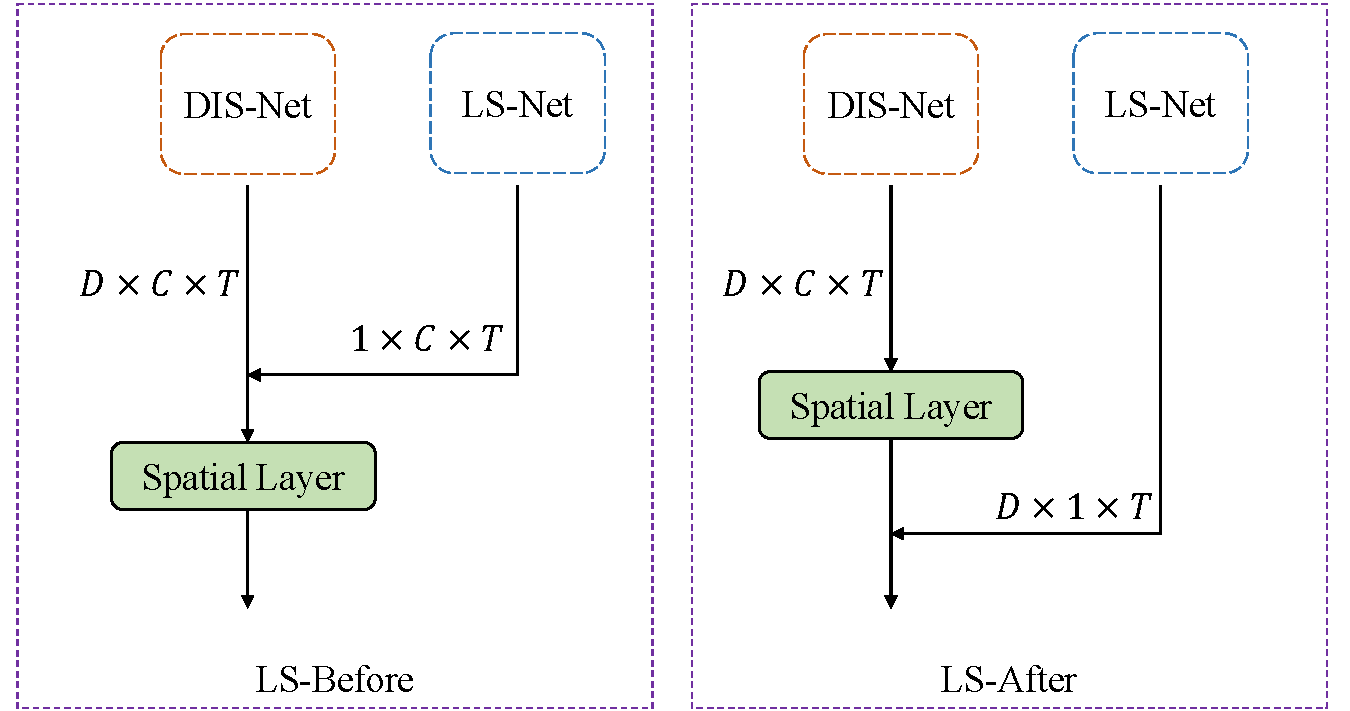
\includegraphics[width=0.6\textwidth]{fuse.pdf}
    \caption{不同融合方式}
    \label{fig:fuse}
\end{figure}

论文在BCI IV 2A数据集上使用HA-FuseNet进行实验,对这两种方式的效果予以验证。实验中对相关超参数进行了固定,从而只关注不同融合方式对性能造成的影响,表~\ref{tab:fuse}~对实验数据进行了展示,其中,准确率与Kappa系数为九位被试的平均表现。
\begin{table}[ht]
    \centering
    \caption{特征融合方式实验结果对比}
    \label{tab:fuse}
    \begin{tabularx}{\textwidth}{CCCC}
      \toprule
      模型 & ACC(\%) & Kappa & SD \\
      \midrule
      LS-After & 76.98 & 0.69 & 10.71 \\
      LS-Before* & \textbf{77.89} & \textbf{0.70} & \textbf{10.22} \\
      \bottomrule
    \end{tabularx}
\end{table}

数据显示,LS-Before具有更高的准确率和一致性,且不同被试的准确率差异较小,这可能是因为LS-Net主要进行了时序特征提取与全局时空自注意力加权两个操作,对空间维度的操作较缺乏,因此需要由空间卷积层进行空间维度的特征提取,以获得更丰富的特征表达;而LS-After将空间维度的特征视为深度维度,可能造成了特征之间的混淆,因此反而不利于提高分类的精确度。论文采用LS-Before的方式进行LS-Net和DIS-Net的特征融合。

\subsection{各模块消融实验}

为了探究论文所提出的各个模块的有效性,并研究不同模块对HA-FuseNet分类效果的影响,论文针对这些模块进行消融实验,按照模型构建的顺序,从基准模型开始,逐步对新增模块后的模型效果进行实验验证。

论文对不同结构的模型作以下定义:

(1) Inception:针对EEG信号的特点,修改了卷积核的基础Inception模型,具有三个Inception模块;

(2) Base-Inception:Inception+Bottleneck,即论文所提出的BaseNet。在Inception模型的基础上引入反转瓶颈层,并对分支数量、激活函数等进行了调整,同时,针对EEG信号的特性,对卷积核大小进行了调整;

(3) BI+Dense:Inception+Bottleneck+Dense Block,即论文所提出的DI-Net。在BaseNet的基础上,引入了密集连接模块;

(4) DI+svSE:Inception+Bottleneck+Dense Block+svSE,即论文所提出的DIS-Net。在DI-Net的基础上,引入了svSE混合注意力模块;

(5) DIS+LSTM:Inception+Bottleneck+Dense Block+svSE+LSTM。在DIS-Net的基础上,引入了LSTM网络;

(6) DIS+LSTM+SCoT:Inception+Bottleneck+Dense Block+svSE+LSTM+SCoT,即论文所提出的结合了DIS-Net和LS-Net的HA-FuseNet。在DIS+LSTM的基础上,引入了SCoT全局自注意力模块。

论文在BCI IV 2A数据集上进行消融实验,表~\ref{tab:ab}~展示了实验的结果,其中,准确率和Kappa系数是九位被试的平均结果。

\begin{table}[ht]
    \centering
    \caption{HA-FuseNet各模块消融实验结果对比}
    \label{tab:ab}
    \begin{tabularx}{\textwidth}{CCCC}
      \toprule
      模型 & ACC(\%) & Kappa & SD \\
      \midrule
      Inception &67.40&0.56&16.15\\
      Base-Inception &72.35&0.63&12.27\\
      BI+Dense &74.42&0.65& 11.92\\
      DI+svSE &76.16&0.68&11.33\\
      DIS+LSTM &76.78 &0.69 & 10.72\\
      DIS+LSTM+SCoT* &\textbf{77.89}&\textbf{0.70}&\textbf{10.22} \\
      \bottomrule
    \end{tabularx}
\end{table}

实验数据显示,Inception+Bottleneck+Dense Block+svSE+LSTM+SCoT结构,即本文所提出的最终模型HA-FuseNet在MI-EEG分类任务上表现最好,准确率、Kappa一致性系数分别达到了77.89\%、0.70,标准差达到了10.22,证明在不同被试上,HA-FuseNet取得了最好的分类性能,且被试之间的准确率差异较小,具有较好的稳定性。

随着模型的逐渐复杂,准确率、Kappa一致性呈现上升趋势,标准差呈现下降趋势,证明了每个模块的有效性。此外,对Inception进行MI-EEG分类任务的针对性改进后得到的BaseNet具有最明显的提升,此后依次为多尺度密集连接模块、svSE模块、SCoT模块、LSTM模块。从对最终模型的贡献度来看,可能说明了相较于循环神经网络,卷积神经网络在MI-EEG分类任务上具有更大的优势。

实验证明了论文所提出的各个模块的有效性,这些模块共同构成了最终模型HA-FuseNet,在BCI IV 2A数据集上取得了77.89\%的平均准确率和0.70的平均Kappa一致性系数。在后续实验中,使用完整的模型。

\subsection{BCI Competition IV Dataset 2A数据集上的对比实验}

在相同的实验设置下,论文在BCI Competition IV Dataset 2A数据集上进行HA-FuseNet与主流模型的被试内(Subject Dependent)对比实验和被试间(Subject Independent)对比实验,以对HA-FuseNet相对于其他模型在MI-EEG分类任务中的性能进行评估。

论文所使用的与HA-FuseNet进行对比的模型中,ShallowConvNet\cite{schirrmeister2017deep}与DeepConvNet\cite{schirrmeister2017deep}是基于卷积神经网络搭建;EEGNet\cite{lawhern2018eegnet}参考了BCI领域经典算法FBCSP的思想,将深度可分离卷积引入了网络结构中;EEGResNet\cite{HBM:HBM23730}基于残差神经网络\cite{he2016deep}构建;EEGInception\cite{zhang2021eeg}使用了Inception多分支和残差连接;EEGConformer\cite{song2022eeg}使用Transformer\cite{vaswani2017attention}与卷积神经网络串联,用以EEG信号的解码;LMDA-Net\cite{miao2023lmda}提出了一种新颖的通道注意力模块和深度注意力模块,基于ShallowConvNet和EEGNet进行了改进。

对于BCI Competition IV Dataset 2A数据集,实验数据显示:

(1) HA-FuseNet在未进行数据增强的被试内实验中,取得了最优的准确率和Kappa一致性,且准确率标准差达到了10.22,证明了HA-FuseNet具有优秀的MI-EEG分类能力,且对不同的被试具有较好的稳定性;

(2) 使用SG轻量化卷积模块的HA-FuseNet(SG)在未进行数据增强的被试内实验中,尽管性能较HA-FuseNet有所下降,但准确率和Kappa系数仅次于ShallowConvNet,且标准差低于ShallowConvNet,HA-FuseNet(SG)的平均准确率较HA-FuseNet下降了约0.66个百分点,在一些被试上,其准确率高于HA-FuseNet;

(3) HA-FuseNet在被试间实验中,取得了最高的平均准确率和Kappa一致性,证明了HA-FuseNet具有优秀的跨被试泛化能力。

实验结果证实,论文所提出的模型HA-FuseNet具有一定的有效性,能够使用较小规模的数据集取得优秀的性能表现,且具有相较于基准模型最优的分类精度和跨被试泛化能力,而使用数据增强算法后,HA-FuseNet的性能表现能够得到进一步的增强。

\paragraph{被试内对比实验}

BCI IV 2A数据集共有九名被试,每名被试具有独立的训练集和测试集,被试内对比实验即使用每名被试对应的训练集和测试集,即为每名被试训练了一个模型。

表~\ref{tab:2acomparein}~展示了不同模型进行被试内实验的准确率,最后一列为九名被试的准确率均值,表~\ref{tab:2acompareinsd}~展示了被试内实验的Kappa一致性系数和标准差,其中,Kappa一致性系数为九名被试的平均值,标准差为准确率标准差。为了更直观地对数据进行展示,在表~\ref{tab:2acomparein}~和表~\ref{tab:2acompareinsd}~中通过加粗的方式对最优值进行了强调。此外,使用*号注明论文所提出的方法。在后文中,延续这些表格设置方法。

需要说明的是,表~\ref{tab:2acomparein}~和~\ref{tab:2acompareinsd}~展示的是未进行数据增强的结果,即对于每名被试,使用数据规模为288的训练集。

\begin{table}[ht]
    \centering
    \caption{HA-FuseNet与基准模型在2A数据集上的被试内实验结果对比(Acc\%)}
    \label{tab:2acomparein}
    \begin{subtable}[ht]{\textwidth}
      \centering
    %   \caption{子表a}
      \label{tab:2acompareina}
      \begin{tabularx}{\textwidth}{cCCCCC}
        \toprule
        \multirow{2}{*}{模型} &  \multicolumn{5}{c}{被试}\\
        \cline{2-6}
         & 1 & 2 & 3 & 4 & 5\\
        \midrule
        ShallowConvNet\cite{schirrmeister2017deep}  & 84.03 & 61.46 & \textbf{94.10} & \textbf{70.83} & 73.26 \\
        DeepConvNet\cite{schirrmeister2017deep} & 83.68 & \textbf{65.28} & 90.63 & 69.44 & \textbf{76.04} \\
        EEGNet\cite{lawhern2018eegnet} & 78.13 & 63.54 & 82.30 & 60.42 & 71.88 \\
        EEGResNet\cite{HBM:HBM23730} & 69.10 & 40.97 & 63.89 & 49.65 & 45.49 \\
        EEGInception\cite{zhang2021eeg} & 71.18 & 48.26 & 82.29 & 55.90 & 64.58 \\
        EEGConformer\cite{song2022eeg} & 67.71 & 55.21 & 84.72 & 53.82 & 75.69 \\
        LMDA-Net\cite{miao2023lmda} & 86.46 & 60.46 & 90.97 & 59.02 & 69.10 \\
        HA-FuseNet*  & \textbf{87.67} & 62.85 & 92.36 & 67.54 & 75.00\\
        HA-FuseNet(SG)* & 86.81 & 63.89 & 92.01 & 65.54 & 71.88\\
        \bottomrule
      \end{tabularx}
    \end{subtable}
    \begin{subtable}[ht]{\textwidth}
      \centering
    %   \caption{子表b}
      \label{tab:2acompareinb}
      \begin{tabularx}{\textwidth}{cCCCCCC}
        \toprule
        \multirow{2}{*}{模型} &  \multicolumn{4}{c}{被试} & \multirow{2}{*}{均值}\\
        \cline{2-5}
         & 6 & 7 & 8 & 9 &  \\
        \midrule
        ShallowConvNet\cite{schirrmeister2017deep}  & 55.90 & 85.76 & \textbf{89.24} & \textbf{85.42} & 77.78 \\
        DeepConvNet\cite{schirrmeister2017deep} & 64.58 & 89.93 & 79.51 & 73.61 & 76.97 \\
        EEGNet\cite{lawhern2018eegnet} & 59.03 & 72.92 & 68.06 & 66.67 & 69.21 \\
        EEGResNet\cite{HBM:HBM23730} & 42.36 & 54.51 & 61.11 & 64.93 & 54.67 \\
        EEGInception\cite{zhang2021eeg} & 52.43 & 75.00 & 85.41 & 73.61 & 67.63 \\
        EEGConformer\cite{song2022eeg} & 53.47 & 69.10 & 71.53 & 58.68 & 65.55 \\
        LMDA-Net\cite{miao2023lmda} & 55.90 & 90.28 & 81.94 & 76.04 & 74.50 \\
        HA-FuseNet*  & \textbf{65.97} & 89.58 & 81.60 & 78.47 & \textbf{77.89} \\
        HA-FuseNet(SG)*  & 62.85 & \textbf{91.67} & 83.68 & 74.95 & 77.23 \\
        \bottomrule
      \end{tabularx}
    \end{subtable}
\end{table}
\begin{table}[ht]
    \centering
    \caption{HA-FuseNet与基准模型在2A数据集上的被试内实验结果对比(Kappa/SD)}
    \label{tab:2acompareinsd}
    \begin{tabularx}{\textwidth}{CCC}
      \toprule
      模型 & Kappa & SD\\
      \midrule
      ShallowConvNet\cite{schirrmeister2017deep} & 0.69 & 12.35\\
      DeepConvNet\cite{schirrmeister2017deep} & 0.69 & 9.22 \\
      EEGNet\cite{lawhern2018eegnet} & 0.60 & \textbf{7.40} \\
      EEGResNet\cite{HBM:HBM23730} & 0.36 & 9.94 \\
      EEGInception\cite{zhang2021eeg} & 0.56 & 12.41 \\
      EEGConformer\cite{song2022eeg} & 0.53 & 10.33 \\
      LMDA-Net\cite{miao2023lmda} & 0.65 & 13.01 \\
      HA-FuseNet* &\textbf{0.70}&10.22\\
      HA-FuseNet(SG)* &0.69&11.14\\
      \bottomrule
    \end{tabularx}
\end{table}

对比基准模型的实验数据,可以发现以下结果:

(1) 对于基准模型,ShallowConvNet取得了最高的平均准确率与Kappa值,但准确率标准差达到了12.35,表明不同被试之间的准确率差异较为明显,性能相对不均衡;

(2) EEGNet取得了最优的准确率标准差,表明不同被试之间准确率差异较小,性能比较均衡,但平均准确率与Kappa值分别为69.21\%、0.60,低于ShallowConvNet、DeepConvNet和LMDA-Net;

(3) LMDA-Net的平均准确率与Kappa值仅低于ShallowConvNet、DeepConvNet,但取得了最高的准确率标准差,表明不同被试之间准确率差异最为明显,由于LMDA-Net是基于EEGNet和ShallowConvNet的改进,这种差异主要可能来源于LMDA-Net提出的局部通道注意力与深度注意力机制,对不同被试特征的关注能力较为不均衡;

(4) EEGResNet取得了最差的效果,低于EEGConformer,这可能是因为在未进行数据增强的情况下,EEGResNet无法很好地发挥其深度架构的优势,而EEGConformer使用了未经过预训练的Transformer,这可能成为其在较小规模的数据集上表现不优的原因;

对比基准模型和论文提出的模型的实验数据,可以发现HA-FuseNet取得了最高的平均准确率和Kappa值,且在1号被试和6号被试上取得了最高的准确率,对于其他模型平均表现较差的2号和4号被试,HA-FuseNet也取得了良好的性能。同时,HA-FuseNet的准确率标准差低于具有次优平均准确率和Kappa值的ShallowConvNet;使用SG轻量化卷积模块的HA-FuseNet(SG)取得了仅次于ShallowConvNet的准确率和Kappa一致性,其准确率的标准差同样低于ShallowConvNet。相较于HA-FuseNet,HA-FuseNet(SG)的平均准确率仅下降了约0.66个百分点。

实验证明了HA-FuseNet和HA-FuseNet(SG)的有效性,能够在使用小规模数据集的情况下取得较好的性能表现。此外,通过对各项模型的实验结果分析,印证了先前研究中,关于浅层网络在小规模数据集的MI-EEG分类任务中性能表现优良的理论,而多尺度密集连接使得HA-FuseNet能够同时利用多尺度的低级特征和高级语义信息,同时,通过全局自注意力机制和局部混合注意力机制进行多维的加权,利用LSTM对时间维度的长短期依赖关系进行提取,综合取得了较基准模型更好的性能。

\paragraph{数据增强被试内对比实验}

论文采用数据增强算法对训练集进行扩充,并扩充至原本的四倍(其中包括原始数据)。需要说明的是,进行数据增强算法延长了模型的训练时间,增大了计算消耗。

表~\ref{tab:2acompareag}~展示了进行数据增强后各模型在BCI IV 2A数据集上进行被试内实验的准确率,表~\ref{tab:2acompareagsd}~则展示了Kappa系数和标准差的对比结果。

数据显示,除EEGConformer之外,其他模型的平均准确率均有所上升,其中,EEGInception的平均准确率升高了10.79个百分点,EEGResNet升高了约9.9个百分点,DeepConvNet和HA-FuseNet的平均准确率上升幅度则相对较小,但论文研究的重点在于基于小规模数据集的MI-EEG分类,因此并无太大影响。这证明了数据增强算法的有效性,可以基于此增加模型学习不同频带数据分布的能力,从而提升模型的性能表现。

值得注意的是,EEGConformer的性能反而出现了下降,这说明基于频率混叠的数据增强算法或许并不适用于Transformer架构,这可能说明了EEGConformer将Transformer直接引入卷积层之后形成串联模型的方式具有受限的提取不同频率成分的能力。如果要将Transformer应用于MI-EEG分类任务中,采用合适的滤波器进行数据预处理,并基于其他方法进行数据增强从而形成较大规模的数据集,可能是更适合的方法,例如,在EEGConformer论文中,使用了基于滑动窗口的数据增强方法\cite{song2022eeg}。

\begin{table}[ht]
    \centering
    \caption{基于数据增强的HA-FuseNet与基准模型在2A数据集上的被试内实验结果对比(Acc\%)}
    \label{tab:2acompareag}
    \begin{subtable}[ht]{\textwidth}
      \centering
    %   \caption{子表a}
      \label{tab:2acompareaga}
      \begin{tabularx}{\textwidth}{CCCCCC}
        \toprule
        \multirow{2}{*}{模型} &  \multicolumn{5}{c}{被试}\\
        \cline{2-6}
         & 1 & 2 & 3 & 4 & 5\\
        \midrule
        ShallowConvNet\cite{schirrmeister2017deep}  & 89.72 & 66.20 & 94.34 & \textbf{84.54} & \textbf{76.39} \\
        DeepConvNet\cite{schirrmeister2017deep} & 82.58 & 62.37 & 91.11 & 73.14 & 69.18 \\
        EEGNet\cite{lawhern2018eegnet} & 77.61 & 67.77 & \textbf{94.95} & 66.25 & 61.63 \\
        EEGResNet\cite{HBM:HBM23730} & 77.88 & 53.05 & 76.22 & 65.37 & 49.39 \\
        EEGInception\cite{zhang2021eeg}  & 88.07 & 61.93 & 91.29 & 77.83 & 69.97 \\
        EEGConformer\cite{song2022eeg}  & 80.05 & 47.82 & 85.98 & 25.27 & 58.25 \\
        LMDA-Net\cite{miao2023lmda} & 88.15 & \textbf{69.16} & 91.99 & 81.18 & 70.31 \\ 
        HA-FuseNet* & \textbf{90.37} & 67.85 & 94.36 & 72.14 & 77.08\\
        \bottomrule
      \end{tabularx}
    \end{subtable}
    \begin{subtable}[ht]{\textwidth}
      \centering
    %   \caption{子表b}
      \label{tab:2acompareagb}
      \begin{tabularx}{\textwidth}{CCCCCCC}
        \toprule
        \multirow{2}{*}{模型} &  \multicolumn{4}{c}{被试} & \multirow{2}{*}{均值}\\
        \cline{2-5}
         & 6 & 7 & 8 & 9 &  \\
        \midrule
        ShallowConvNet\cite{schirrmeister2017deep}  & \textbf{62.24} & \textbf{96.69} & \textbf{90.94} & \textbf{89.55} & \textbf{83.40} \\
        DeepConvNet\cite{schirrmeister2017deep}  & 59.38 & 86.85 & 85.80 & 82.58 & 77.00 \\
        EEGNet\cite{lawhern2018eegnet} & 46.09 & 85.80 & 83.71 & 87.63 & 74.61 \\
        EEGResNet\cite{HBM:HBM23730}  & 44.44 & 77.61 & 75.35 & 61.85 & 64.57 \\
        EEGInception\cite{zhang2021eeg} & 57.03 & 90.33 & 84.76 & 84.58 & 78.42 \\
        EEGConformer\cite{song2022eeg}  & 26.65 & 52.27 & 27.00 & 25.61 & 47.65 \\
        LMDA-Net\cite{miao2023lmda}& 60.24 & 93.21 & 83.28 & 86.41 & 80.44 \\ 
        HA-FuseNet* & 67.92 & 93.75 & 83.68 & 87.15 & 81.56 \\
        \bottomrule
      \end{tabularx}
    \end{subtable}
\end{table}
\begin{table}[H]
    \centering
    \caption{基于数据增强的HA-FuseNet与基准模型在2A数据集上的被试内实验结果对比(Kappa/SD)}
    \label{tab:2acompareagsd}
    \begin{tabularx}{\textwidth}{CCC}
      \toprule
      模型 & Kappa & SD \\
      \midrule
      ShallowConvNet\cite{schirrmeister2017deep} & \textbf{0.78} & 11.67 \\
      DeepConvNet\cite{schirrmeister2017deep} & 0.69 & 10.73 \\
      EEGNet\cite{lawhern2018eegnet} & 0.66 & 14.52 \\
      EEGResNet\cite{HBM:HBM23730} & 0.53 & 12.36 \\
      EEGInception\cite{zhang2021eeg} & 0.71 & 11.92 \\
      EEGConformer\cite{song2022eeg} & 0.30 & 22.38 \\
      LMDA-Net\cite{miao2023lmda} & 0.74 & 10.74 \\
      HA-FuseNet* & 0.76 & \textbf{10.09} \\
      \bottomrule
    \end{tabularx}
\end{table}

此外,表~\ref{tab:2acompareagsd}~表明进行数据增强之后,除EEGConformer之外,其他模型的Kappa一致性均有所上升。论文所提出的HA-FuseNet的Kappa值达到了0.76,准确率的标准差下降为10.09,标准差为所有模型中的最低值,表明HA-FuseNet的在不同被试间的稳定性得到了进一步的加强。

\paragraph{被试间对比实验}

在被试间对比实验中,对于被试\(i\),使用全部其他被试的训练集为被试\(i\)的训练集,如公式~\ref{eq:cross}~所示,其中,\(Train_j\)表示被试\(j\)的训练集。仍然使用被试\(i\)的测试集为测试集。
\begin{equation}
    \label{eq:cross}
    Train_i=\sum_{j}^{9}Train_j,\,i \in (1,2,...,9),\,j \in (1,2,...,9),\,j \neq i
\end{equation}

表~\ref{tab:2acomparecross}~展示了各个模型进行被试间实验的准确率结果对比,例如,表格中[ShallowConvNet,1]即表示ShallowConvNet使用其他八名被试的训练集集合,在1号被试的测试集上得到的准确率。表~\ref{tab:2acomparecrosssd}~展示了被试间实验的Kappa系数和标准差结果对比。被试间对比实验未使用数据增强算法。

对比基准模型的实验数据,可以发现以下结果:

(1) DeepConvNet在基准模型中具有最高的平均准确率和Kappa系数,准确率标准差达到了9.54,DeepConvNet在被试间实验中取得了优于ShallowConvNet的性能,这可能是因为DeepConvNet学习到了更为抽象和高级的特征,从而更好地适应了不同被试间的数据差异;

(2) EEGNet取得了最优的准确率标准差,但平均准确率和Kappa值为63.23\%、0.51,仅优于EEGResNet和EEGConformer,这说明了EEGNet具有较好的稳定性,但分类的准确率和一致性较差;

(3) 所有基准模型在被试2号、4号、6号的跨被试实验中,平均性能表现较差。

对比基准模型和论文提出的模型的实验数据,可以发现论文提出的HA-FuseNet取得了最优的平均准确率和Kappa系数,且平均准确率比DeepConvNet提升了约0.63\%,HA-FuseNet的准确率标准差达到了11.06,仅比DeepConvNet上升了约0.52。

此外,论文提出的HA-FuseNet在被试1、2、3、7、8、9号上的表现优于DeepConvNet,仅在被试4、5、6号上的表现低于DeepConvNet。但应当注意到,在基准模型平均性能较差的被试2、4、6号上,HA-FuseNet取得了较为均衡的分类精度,在被试2号中,HA-FuseNet的精度仅低于EEGNet,被试4号中,仅低于DeepConvNet和EEGNet。

实验证实了论文提出的HA-FuseNet在具有22通道的BCI IV 2A数据集上具有良好的分类性能和跨被试泛化能力,能够满足论文的研究目标。

\begin{table}[H]
    \centering
    \caption{HA-FuseNet与基准模型在2A数据集上的被试间实验结果对比(Acc\%)}
    \label{tab:2acomparecross}
    \begin{subtable}[ht]{\textwidth}
      \centering
    %   \caption{子表a}
      \label{tab:2acomparecrossa}
      \begin{tabularx}{\textwidth}{CCCCCC}
        \toprule
        \multirow{2}{*}{模型} &  \multicolumn{5}{c}{被试}\\
        \cline{2-6}
         & 1 & 2 & 3 & 4 & 5\\
        \midrule
        ShallowConvNet\cite{schirrmeister2017deep}   & \textbf{76.39} & 47.92 & \textbf{88.54} & 55.56 & 57.64\\
        DeepConvNet\cite{schirrmeister2017deep} & 71.53 & 50.69 & 84.72 & \textbf{61.46} & \textbf{69.10} \\
        EEGNet\cite{lawhern2018eegnet} & 68.75 & \textbf{56.60} & 68.75 & 61.11 & 68.75 \\
        EEGResNet\cite{HBM:HBM23730} & 61.81 & 38.54 & 64.24 & 45.83 & 39.93 \\
        EEGInception\cite{zhang2021eeg}  & 74.31 & 51.04 & 81.60 & 52.43 & 56.25 \\
        EEGConformer\cite{song2022eeg}  & 52.78 & 26.04 & 26.04 & 50.00 & 64.24\\
        LMDA-Net\cite{miao2023lmda} & 72.22 & 47.22 & 83.68 & 55.90 & 51.74 \\ 
        HA-FuseNet*  & 76.13 & 52.79 & 86.89 & 57.13 & 60.42\\
        \bottomrule
      \end{tabularx}
    \end{subtable}
    \begin{subtable}[ht]{\textwidth}
      \centering
    %   \caption{子表b}
      \label{tab:2acomparecrossb}
      \begin{tabularx}{\textwidth}{CCCCCCC}
        \toprule
        \multirow{2}{*}{模型} &  \multicolumn{4}{c}{被试} & \multirow{2}{*}{均值}\\
        \cline{2-5}
         & 6 & 7 & 8 & 9 &  \\
        \midrule
        ShallowConvNet\cite{schirrmeister2017deep}  & 55.21 & 74.65 & \textbf{81.25} & 72.92 & 67.79 \\
        DeepConvNet\cite{schirrmeister2017deep}  & 59.03 & 75.35 & 74.31 & 64.93 & 67.90 \\
        EEGNet\cite{lawhern2018eegnet}  & 58.68 & 73.61 & 56.60 & 56.25 & 63.23 \\
        EEGResNet\cite{HBM:HBM23730}  & 42.01 & 47.22 & 50.69 & 56.25 & 49.61 \\
        EEGInception\cite{zhang2021eeg}  & \textbf{60.42} & 71.18 & 73.96 & \textbf{74.31} & 66.17 \\
        EEGConformer\cite{song2022eeg} & 25.00 & 26.74 & 29.51 & 27.78 & 36.46\\
        LMDA-Net\cite{miao2023lmda}  & 48.26 & 71.88 & 76.04 & 66.67 & 63.73\\
        HA-FuseNet*  & 58.49 & \textbf{76.74} & 78.13 & 70.06 & \textbf{68.53} \\
        \bottomrule
      \end{tabularx}
    \end{subtable}
\end{table}
\begin{table}[ht]
    \centering
    \caption{HA-FuseNet与基准模型在2A数据集上的被试间实验结果对比(Kappa/SD)}
    \label{tab:2acomparecrosssd}
    \begin{tabularx}{\textwidth}{CCC}
      \toprule
      模型 & Kappa & SD \\
      \midrule
      ShallowConvNet\cite{schirrmeister2017deep} &0.57&13.19 \\
      DeepConvNet\cite{schirrmeister2017deep} &0.57 &9.54\\
      EEGNet\cite{lawhern2018eegnet} &0.51& \textbf{6.33}\\
      EEGResNet\cite{HBM:HBM23730} &0.33&8.83\\
      EEGInception\cite{zhang2021eeg} &0.55&10.57\\
      EEGConformer\cite{song2022eeg}&0.15&14.09 \\
      LMDA-Net\cite{miao2023lmda} &0.52&12.53\\
      HA-FuseNet* &\textbf{0.57}&11.06\\
      \bottomrule
    \end{tabularx}
\end{table}


\subsection{BCI Competition IV Dataset 2B数据集上的对比实验}

为了评估论文所提出的模型在不同硬件设施(电极数量)的场景下的性能,论文在BCI Competition IV Dataset 2B数据集上进行HA-FuseNet与主流模型的被试内和被试间对比实验。相较于BCI IV 2A数据集的22通道,BCI IV 2B数据集仅使用3个通道记录EEG数据,对模型在较低空间分辨率条件下的性能提出了挑战。BCI IV 2B数据集上的实验未进行数据增强,以对模型在小规模数据集上的表现进行评估。

论文所使用的与HA-FuseNet进行对比的基准模型与前文相同,包括ShallowConvNet\cite{schirrmeister2017deep}、DeepConvNet\cite{schirrmeister2017deep}、EEGNet\cite{lawhern2018eegnet}、EEGResNet\cite{HBM:HBM23730}、EEGInception\cite{zhang2021eeg}、EEGConformer\cite{song2022eeg}和LMDA-Net\cite{miao2023lmda}。

对于BCI Competition IV Dataset 2B数据集,实验数据显示HA-FuseNet在被试内实验和被试间实验中,均取得了最优的平均准确率和Kappa一致性。在被试内实验中,HA-FuseNet的平均准确率、Kappa系数和准确率标准差分别达到了75.23\%、0.50和8.84,其中,准确率标准差仅高于具有较差性能表现的EEGResNet。在被试间实验中,HA-FuseNet的平均准确率、Kappa系数和准确率标准差分别达到了76.86\%、0.53和6.68,其中,准确率标准差仅高于性能表现最差的EEGConformer。

实验结果证明了论文所提出的HA-FuseNet具有良好的适应低空间分辨率场景的能力,其具有优秀的分类精度和分类一致性,在不同被试上具有稳定的泛化能力,同时,HA-FuseNet对数据增强算法没有强依赖性,在小规模数据集上也表现出优秀的性能。

\paragraph{被试内对比实验}

BCI IV 2B数据集共有九名被试,被试内对比实验即对每名被试,使用其训练集和测试集数据进行独立的训练和测试。

表~\ref{tab:2bcomparein}~展示了HA-FuseNet和基准模型进行被试内实验的准确率。表~\ref{tab:2bcompareinsd}~展示了各个模型进行被试内实验的Kappa一致性系数和准确率的标准差。

对比基准模型的实验数据,可以发现以下结果:

(1) EEGInception在基准模型中具有最高的平均准确率和Kappa系数,其表现超过了ShallowConvNet,后者在BCI IV 2A数据集上具有最优的准确率和一致性表现。这说明了EEGInception具有更好的适应低空间分辨率场景的能力,而ShallowConvNet的适应性则有所下降,这种差异可能来源于二者的架构差别,EEGInception着重提取时间维度特征,而ShallowConvNet对时域和空域的特征应用了相同的策略;

(2) EEGResNet取得了最优的准确率标准差,表明在不同被试之间的性能较为稳定,然而,EEGResNet的平均准确率为68.51\%,相较于EEGInception降低了6.07个百分点,说明其分类精度相对较差;

(3) BCI IV 2A数据集上,各个基准模型取得的平均准确率的均值约为69.47\%,高于平均值的模型有ShallowConvNet、DeepConvNet和LMDA-Net;BCI IV 2B数据集上,各个基准模型取得的平均准确率的均值约为70.74\%,高于平均值的模型有DeepConvNet、EEGInception和LMDA-Net;此外,相较于BCI IV 2A数据集,EEGResNet、EEGConformer在BCI IV 2B数据集上的准确率更接近均值,EEGNet落后均值的幅度增加,DeepConvNet、LMDA-Net领先均值的幅度则降低了。这或许说明了空间分辨率较高时,EEG信号特征明显,因此浅层网络就能够取得较好的效果,而空间分辨率较低时,需要更为复杂的网络提取EEG信号的特征。此外,LMDA-Net证明了针对EEG信号特性设计的注意力模块能够取得良好的效果。

\begin{table}[ht]
    \centering
    \caption{HA-FuseNet与基准模型在2B数据集上的被试内实验结果对比(Acc\%)}
    \label{tab:2bcomparein}
    \begin{subtable}[ht]{\textwidth}
      \centering
    %   \caption{子表a}
      \label{tab:2bcompareina}
      \begin{tabularx}{\textwidth}{CCCCCC}
        \toprule
        \multirow{2}{*}{模型} &  \multicolumn{5}{c}{被试}\\
        \cline{2-6}
         & 1 & 2 & 3 & 4 & 5\\
        \midrule
        ShallowConvNet\cite{schirrmeister2017deep}  & 78.33 & 74.17 & 59.17 & 90.77 & 63.08\\
        DeepConvNet\cite{schirrmeister2017deep}  & 78.33 & 72.50 & 59.17 & \textbf{97.69} & 68.46\\
        EEGNet\cite{lawhern2018eegnet}  & 78.33 & 73.33 & 60.00 & 94.61 & 59.23 \\
        EEGResNet\cite{HBM:HBM23730}  & 68.33 & 62.50 & 58.33 & 87.69 & 70.00 \\
        EEGInception\cite{zhang2021eeg}  & \textbf{81.67} & 70.83 & 63.33 & 90.00 & \textbf{82.31} \\
        EEGConformer\cite{song2022eeg}  & 72.50 & 73.33 & 60.00 & 88.46 & 56.92\\
        LMDA-Net\cite{miao2023lmda}  & 76.67 & 75.00 & 65.00 & 93.85 & 64.61 \\
        HA-FuseNet*   & 79.17 & \textbf{80.00} & \textbf{70.83} & 95.39 & 76.92 \\
        \bottomrule
      \end{tabularx}
    \end{subtable}
    \begin{subtable}[ht]{\textwidth}
      \centering
    %   \caption{子表b}
      \label{tab:2bcompareinb}
      \begin{tabularx}{\textwidth}{CCCCCCC}
        \toprule
        \multirow{2}{*}{模型} &  \multicolumn{4}{c}{被试} & \multirow{2}{*}{均值}\\
        \cline{2-5}
         & 6 & 7 & 8 & 9 &  \\
        \midrule
        ShallowConvNet\cite{schirrmeister2017deep}  & 80.83 & 68.33 & 59.29 & 60.83 & 70.53 \\
        DeepConvNet\cite{schirrmeister2017deep}  & 80.00 & \textbf{76.67} & 63.57 & 60.00 & 72.93 \\
        EEGNet\cite{lawhern2018eegnet}  & 66.67 & 72.50 & 57.86 & 57.50 & 68.89 \\
        EEGResNet\cite{HBM:HBM23730}  & 73.33 & 67.50 & 66.43 & 62.50 & 68.51\\
        EEGInception\cite{zhang2021eeg}  & \textbf{81.67} & 69.17 & 66.43 & \textbf{65.83} & 74.58 \\
        EEGConformer\cite{song2022eeg}  & 70.83 & 70.83 & 60.71 & 60.83 & 68.27\\
        LMDA-Net\cite{miao2023lmda}  & 80.00 & 70.83 & 60.71 & 56.67 & 71.48 \\
        HA-FuseNet*   & 75.00 & 69.17 & \textbf{66.43} & 64.17 & \textbf{75.23} \\
        \bottomrule
      \end{tabularx}
    \end{subtable}
\end{table}
\begin{table}[H]
    \centering
    \caption{HA-FuseNet与基准模型在2B数据集上的被试内实验结果对比(Kappa/SD)}
    \label{tab:2bcompareinsd}
    \begin{tabularx}{\textwidth}{CCC}
      \toprule
      模型 & Kappa & SD \\
      \midrule
      ShallowConvNet\cite{schirrmeister2017deep} &0.41&10.54\\
      DeepConvNet\cite{schirrmeister2017deep} &0.45&11.40\\
      EEGNet\cite{lawhern2018eegnet} &0.38& 11.61\\
      EEGResNet\cite{HBM:HBM23730} &0.37&\textbf{7.99}\\
      EEGInception\cite{zhang2021eeg} &0.49&8.89\\
      EEGConformer\cite{song2022eeg} &0.36&9.27\\
      LMDA-Net\cite{miao2023lmda} &0.43&10.73\\
      HA-FuseNet* &\textbf{0.50}&8.84\\
      \bottomrule
    \end{tabularx}
\end{table}

基准模型的实验结果印证了论文设计模型的思路的正确性,包括更关注时间维度特征、同时利用深层和浅层特征、针对EEG信号特性设计注意力模块等。这些设计使得HA-FuseNet对空间分辨率具有低依赖性,即对于高空间分辨率和低空间分辨率的场景,都能取得较好的性能表现。

实验数据证实,相较于基准模型,HA-FuseNet取得了最高的平均准确率和Kappa值,分别达到了75.23\%和0.50,在被试2、3、8号上取得了所有模型中最优的准确率,且在被试4、7号上取得了高于或持平于次优模型EEGInception的准确率。HA-FuseNet的准确率标准差达到了8.84,优于EEGInception,仅次于EEGResNet,证明HA-FuseNet不仅具有优秀的分类精度,同时在不同被试间具有良好的稳定性。

\paragraph{被试间对比实验}

被试间对比实验中,对于一名被试,使用其他所有被试的训练集为该被试的训练集,即训练集的数据规模为\(120\times8\),测试集为该被试的测试集,数据规模仍然为120。

表~\ref{tab:2bcomparecross}~展示了BCI IV 2B数据集上HA-FuseNet和基准模型进行被试间实验的准确率。表~\ref{tab:2bcomparecrosssd}~展示了被试间实验的Kappa一致性系数和准确率标准差。

对比基准模型的实验数据,可以发现以下结果:

(1) EEGInception在基准模型之中具有最优的准确率和Kappa系数,准确率平均值达到了75.64\%,高于次优模型ShallowConvNet大约0.12个百分点;EEGInception的准确率标准差为7.29,约比ShallowConvNet高0.11。这说明EEGInception的分类精度高于ShallowConvNet,但稳定性相对较差。相较于被试内实验,ShallowConvNet在被试间实验中的性能获得了明显的提升,其原因可能是较大的数据规模、较多变的数据分布弥补了ShallowConvNet学习低空间分辨率场景特征能力的不足,相当于ShallowConvNet经过了基于样本集合的数据增强。尽管如此,EEGInception仍然取得了最高的分类精度;

(2) EEGConformer取得了最低的准确率标准差,为6.44,但EEGConformer的平均准确率为基准模型中的最低值,因此,虽然EEGConformer在不同被试之间的稳定性相对较优,但较低的分类精度表明其综合性能仍然较差。

实验数据显示,论文提出的HA-FuseNet的平均准确率和Kappa系数均优于基准模型,分别为76.86\%和0.53,其准确率标准差为6.68,仅高于EEGConformer。然而,考虑到EEGConformer较差的分类精度,仍然可以认为HA-FuseNet的综合性能超过了所有的基准模型。这与在BCI IV 2A数据集上的实验结论相符,HA-FuseNet具有优秀的分类精度和跨被试泛化性能力,且可以使用小规模数据集进行训练,同时,在不同精度的空间分辨率条件下都具有较为稳定的性能。实验证明了HA-FuseNet的有效性。

\begin{table}[h]
    \centering
    \caption{HA-FuseNet与基准模型在2B数据集上的被试间实验结果对比(Acc\%)}
    \label{tab:2bcomparecross}
    \begin{subtable}[ht]{\textwidth}
      \centering
    %   \caption{子表a}
      \label{tab:2bcomparecrossa}
      \begin{tabularx}{\textwidth}{CCCCCC}
        \toprule
        \multirow{2}{*}{模型} &  \multicolumn{5}{c}{被试}\\
        \cline{2-6}
         & 1 & 2 & 3 & 4 & 5\\
        \midrule
        ShallowConvNet\cite{schirrmeister2017deep}  & 75.00 & 67.50 & 70.83 & \textbf{92.20} & 76.46\\
        DeepConvNet\cite{schirrmeister2017deep}  & 67.50 & 65.00 & 67.50 & 91.54 & 72.31 \\
        EEGNet\cite{lawhern2018eegnet}  & 63.33 & \textbf{70.83} & \textbf{73.33} & 85.39 & 73.85 \\
        EEGResNet\cite{HBM:HBM23730}  & 62.50 & 67.50 & 62.50 & 89.23 & 72.31\\
        EEGInception\cite{zhang2021eeg} & \textbf{77.50} & 63.33 & 72.50 & 87.69 & \textbf{80.00} \\
        EEGConformer\cite{song2022eeg}  & 58.33 & 67.50 & 65.83 & 63.85 & 70.00 \\
        LMDA-Net\cite{miao2023lmda}  & 70.00 & 67.50 & 72.50 & 90.77 & 72.31 \\
        HA-FuseNet*  & 70.80 & 67.50 & 89.23 & 75.39 & 82.50 \\
        \bottomrule
      \end{tabularx}
    \end{subtable}
    \begin{subtable}[ht]{\textwidth}
      \centering
    %   \caption{子表b}
      \label{tab:2bcomparecrossb}
      \begin{tabularx}{\textwidth}{CCCCCCC}
        \toprule
        \multirow{2}{*}{模型} &  \multicolumn{4}{c}{被试} & \multirow{2}{*}{均值}\\
        \cline{2-5}
         & 6 & 7 & 8 & 9 &  \\
        \midrule
        ShallowConvNet\cite{schirrmeister2017deep}  & 81.67 & 75.83 & 70.14 & 70.00 & 75.52 \\
        DeepConvNet\cite{schirrmeister2017deep}  & 86.67 & 76.67 & 70.00 & 70.83 & 74.22 \\
        EEGNet\cite{lawhern2018eegnet}  & 82.50 & \textbf{85.00} & 70.00 & 69.17 & 74.82 \\
        EEGResNet\cite{HBM:HBM23730}  & 78.33 & 69.17 & 69.29 & 65.00 & 70.65 \\
        EEGInception\cite{zhang2021eeg}  & \textbf{85.00} & 74.17 & 71.43 & 69.17 & 75.64 \\
        EEGConformer\cite{song2022eeg}  & 78.33 & 78.33 & 67.86 & 61.67 & 67.97 \\
        LMDA-Net\cite{miao2023lmda}  & 84.17 & 79.17 & 70.71 & 69.17 & 75.14 \\ 
        HA-FuseNet*  & 82.50 & 80.00 & \textbf{72.14} & \textbf{71.67} & \textbf{76.86}\\
        \bottomrule
      \end{tabularx}
    \end{subtable}
\end{table}

\begin{table}[H]
    \centering
    \caption{HA-FuseNet与基准模型在2B数据集上的被试间实验结果对比(Kappa/SD)}
    \label{tab:2bcomparecrosssd}
    \begin{tabularx}{\textwidth}{CCC}
      \toprule
      模型 & Kappa & SD \\
      \midrule
      ShallowConvNet\cite{schirrmeister2017deep} &0.52&7.18\\
      DeepConvNet\cite{schirrmeister2017deep} &0.49& 8.62 \\
      EEGNet\cite{lawhern2018eegnet} &0.51& 7.31\\
      EEGResNet\cite{HBM:HBM23730} &0.39 &8.07\\
      EEGInception\cite{zhang2021eeg} & 0.52 &7.29 \\
      EEGConformer\cite{song2022eeg} &0.35 &\textbf{6.44}\\
      LMDA-Net\cite{miao2023lmda} &0.52&7.43\\ 
      HA-FuseNet* &\textbf{0.53}&6.68\\
      \bottomrule
    \end{tabularx}
\end{table}

\section{本章小结}

本章主要对于第三章构建的MI-EEG分类网络HA-FuseNet进行了消融实验、对比实验和跨被试泛化性实验。首先,介绍了实验使用的软硬件环境。其次,介绍了实验所使用的数据集以及对数据进行处理的方法,同时介绍了实验中所使用的基本配置,包括超参数、损失函数、评估指标等。实验使用BCI Competition IV Dataset 2A数据集和BCI Competition IV Dataset 2B数据集,其具有不同的通道数,能够对模型在不同空间分辨率下的性能进行评估。最后,介绍了具体进行的实验:首先,设计并进行实验,验证不同的网络结构对HA-FuseNet性能的影响,从而选择最合适的架构方式;其次,通过消融实验验证各模块的有效性,讨论每个模块对模型的贡献度;最后,通过在不同数据集上,与当前的多种主流MI-EEG分类模型进行被试内对比实验、被试间对比实验,评估HA-FuseNet的分类精度、被试间稳定性、跨被试泛化性、跨空间分辨率稳定性能力。实验结果证明,HA-FuseNet相较于基准模型取得了综合最优的各项性能,从而证明了论文所提出方法的有效性。